% CameraReady worked example — a short review paper, compiled end to end.
% Build: python scripts/compile_paper.py --project-dir examples/minimal-review-paper
%
% This file is deliberately small. It exists to show what the pipeline
% produces, not to be a publishable survey. See plan/ for the scope decision.

\documentclass[conference]{IEEEtran}
\IEEEoverridecommandlockouts

\usepackage{cite}
\usepackage{amsmath,amssymb,amsfonts}
\usepackage{graphicx}
\usepackage{booktabs}
\usepackage{array}
\usepackage{xcolor}
\usepackage{tikz}
\usepackage{url}
\usetikzlibrary{positioning,arrows.meta}

\definecolor{leverblue}{RGB}{70,130,180}
\definecolor{levergreen}{RGB}{50,150,50}

\begin{document}

\title{From Attention to Adaptation:\\A Short Review of Scaling Levers in Deep Learning}

\author{\IEEEauthorblockN{CameraReady Example}
\IEEEauthorblockA{\textit{Worked example shipped with the CameraReady paper pipeline}\\
\url{https://github.com/e96031413/camera-ready}}}

\maketitle

\begin{abstract}
Deep learning did not scale because of one idea. It scaled because four
separate constraints were removed in sequence: depth was made trainable,
optimization was made robust to hand-tuned learning rates, supervision was
decoupled from the downstream task, and adaptation was decoupled from the full
parameter count. This short review traces those four levers through eight
primary sources and states what each one traded away in return. It is a
worked example for a gated paper-writing pipeline, not a comprehensive survey;
the Limitations section says plainly what eight citations cannot support.
\end{abstract}

\begin{IEEEkeywords}
deep learning, scaling, transformers, pre-training, low-rank adaptation, survey
\end{IEEEkeywords}

\section{Introduction}
\label{sec:intro}

Between 2015 and 2021 the working recipe for a deep learning system changed
almost completely. A practitioner in 2015 designed an architecture for a task,
trained it from scratch on that task's labelled data, and tuned a learning rate
schedule by hand. A practitioner in 2021 downloaded a pre-trained model,
adapted a small fraction of its parameters, and rarely touched the optimizer at
all.

That shift is often narrated as a single story about scale. It is more useful
to read it as four independent constraints being removed, each by a specific
piece of work, and each at a specific cost. Residual connections made depth
trainable~\cite{he2015deepresiduallearningimage}. Attention made sequence
modelling parallel~\cite{vaswani2023attentionneed}. Pre-training decoupled
supervision from the downstream task. Low-rank adaptation decoupled the cost of
specializing a model from its parameter count.

This review covers those four levers and nothing else. Reinforcement learning,
multimodality, and the systems and hardware work that made any of it affordable
are out of scope, and eight citations would not support claims about them.

\section{Architecture and Optimization}
\label{sec:architecture}

The first constraint was depth. Stacking more layers degraded training accuracy,
not just test accuracy, which ruled out overfitting as the explanation. Residual
connections reframed each block as learning a perturbation of the identity
rather than a full transformation, and networks an order of magnitude deeper
became trainable~\cite{he2015deepresiduallearningimage}. The cost was
architectural commitment: the shortcut path constrains what a block may do to
its input.

The second constraint was optimization. Per-parameter adaptive step sizes with
bias-corrected moment estimates removed most of the hand-tuning that a
schedule had previously required~\cite{kingma2017adammethodstochasticoptimization}.
The cost was diagnostic: an optimizer that converges from a poor learning rate
also converges quietly from a poor architecture, which makes a failure harder to
localize.

The third constraint was sequential computation. Recurrence forced a sequence to
be processed in order, so training time scaled with sequence length no matter how
much hardware was available. Replacing recurrence entirely with attention made
the computation parallel across positions~\cite{vaswani2023attentionneed}. The
cost was quadratic: attention compares every position with every other, so memory
grows with the square of the sequence length. Figure~\ref{fig:timeline} places
these three alongside the pre-training work discussed next.

\begin{figure}[t]
\centering
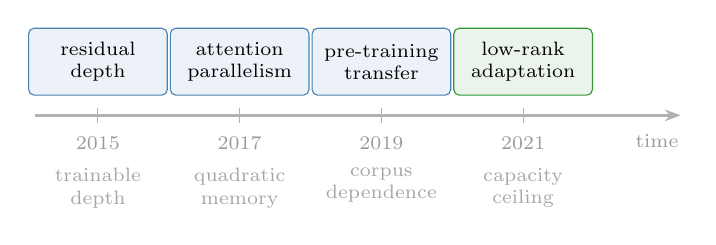
\begin{tikzpicture}[
  every node/.style={font=\scriptsize},
  lever/.style={draw=leverblue, fill=leverblue!10, rounded corners=2pt,
                text width=1.55cm, align=center, inner sep=3pt, minimum height=0.85cm},
  adapt/.style={draw=levergreen, fill=levergreen!10, rounded corners=2pt,
                text width=1.55cm, align=center, inner sep=3pt, minimum height=0.85cm}
]
\draw[-{Stealth[length=2mm]}, gray!60, thick] (-0.3,0) -- (7.9,0);
\node[gray!80, anchor=north] at (7.6,-0.12) {time};

\foreach \x/\y in {0.5/2015, 2.3/2017, 4.1/2019, 5.9/2021} {
  \draw[gray!60] (\x,0.1) -- (\x,-0.1);
  \node[gray!80, anchor=north] at (\x,-0.15) {\y};
}

\node[lever, anchor=south] at (0.5,0.25) {residual\\depth};
\node[lever, anchor=south] at (2.3,0.25) {attention\\parallelism};
\node[lever, anchor=south] at (4.1,0.25) {pre-training\\transfer};
\node[adapt, anchor=south] at (5.9,0.25) {low-rank\\adaptation};

\node[anchor=north, text width=1.55cm, align=center, gray!70] at (0.5,-0.55) {trainable\\depth};
\node[anchor=north, text width=1.55cm, align=center, gray!70] at (2.3,-0.55) {quadratic\\memory};
\node[anchor=north, text width=1.55cm, align=center, gray!70] at (4.1,-0.55) {corpus\\dependence};
\node[anchor=north, text width=1.55cm, align=center, gray!70] at (5.9,-0.55) {capacity\\ceiling};
\end{tikzpicture}
\caption{The four levers, with what each one cost underneath. Dates are the
first arXiv posting of the corresponding work. Drawn in TikZ rather than
included as an image file, so the example compiles from a clean checkout with
no external assets.}
\label{fig:timeline}
\end{figure}

\section{Pre-training and Transfer}
\label{sec:pretraining}

Removing those three constraints made large models trainable. It did not make
them useful, because a large model still needed a large labelled dataset for
each task.

Masked language modelling broke that dependence. Training a bidirectional
encoder to reconstruct masked tokens produces representations that transfer to
tasks the model never saw, and the pre-training signal comes from unlabelled
text~\cite{devlin2019bertpretrainingdeepbidirectional}. The same recipe transfers
across modalities: splitting an image into fixed-size patches and treating them
as a token sequence lets an unmodified transformer encoder compete with
convolutional architectures, provided the pre-training corpus is large
enough~\cite{dosovitskiy2021imageworth16x16words}. Scaling the same objective
further changes the interface rather than only the accuracy: at sufficient
scale, a task can be specified in the prompt instead of through gradient
updates~\cite{brown2020languagemodelsfewshotlearners}.

The cost here is corpus dependence. Each of these results is a claim about a
model \emph{and} the corpus it was pre-trained on, and the two cannot be
separated after the fact. Table~\ref{tab:levers} summarizes the four levers on
that axis.

\begin{table}[t]
\centering
\caption{What each lever changed, and what it cost.}
\label{tab:levers}
% Narrow p{} columns cannot justify without underfull hboxes; ragged right is
% the fix. Note the p{} widths rather than \resizebox: shrinking a table below
% the body font size is a formatting violation at most venues.
\newcolumntype{L}[1]{>{\raggedright\arraybackslash}p{#1}}
\begin{tabular}{@{}L{1.5cm}L{2.6cm}L{2.6cm}@{}}
\toprule
\textbf{Lever} & \textbf{Constraint removed} & \textbf{Cost incurred} \\
\midrule
Residual depth & Deeper networks stopped degrading during training &
Each block is constrained to perturb its input \\
\addlinespace
Attention & Sequence processing became parallel across positions &
Memory grows quadratically with sequence length \\
\addlinespace
Pre-training & Supervision decoupled from the downstream task &
Results are inseparable from the pre-training corpus \\
\addlinespace
Low-rank adaptation & Specialization decoupled from parameter count &
Update capacity bounded by the chosen rank \\
\bottomrule
\end{tabular}
\end{table}

\section{Efficient Adaptation}
\label{sec:adaptation}

Pre-training moved the cost rather than removing it. Adapting a pre-trained
model by full fine-tuning produces a complete copy of its parameters per task,
which becomes the binding constraint once a single model serves many tasks.

Constraining the weight update to a low-rank factorization removes that
constraint: the frozen base model is shared, and each task stores only the small
factors~\cite{hu2021loralowrankadaptationlarge}. The cost is a capacity ceiling
that the practitioner now chooses explicitly. The rank is a hyperparameter, and
too low a rank silently caps how far the adapted model can move from the base.

The same decoupling appears outside language modelling. Diffusion models
separate the generative process into many small denoising steps, each of which
is easy to train, and pay for it in sampling
cost~\cite{ho2020denoisingdiffusionprobabilisticmodels}. The pattern across all
four levers is the same shape: a hard constraint is exchanged for a tunable one.

\section{Discussion and Limitations}
\label{sec:limitations}

Read as a sequence, the four levers are not four solutions. They are four
relocations of the same difficulty. Depth became trainable and the constraint
moved into the block structure. Sequences became parallel and the constraint
moved into memory. Supervision became cheap and the constraint moved into the
corpus. Adaptation became cheap and the constraint moved into a rank
hyperparameter. Each step made the remaining constraint the one the
practitioner chooses rather than the one the method imposes.

\textbf{Limitations.} This review synthesizes eight primary sources. That is
enough to trace an argument and nowhere near enough to survey a field. It omits
reinforcement learning from human feedback, multimodal architectures,
mixture-of-experts routing, quantization, and the systems and hardware work
without which none of these results would have been reachable. It reports no
benchmark numbers, because we reproduced none of them, and it takes each paper's
own account of its contribution at face value rather than re-evaluating it.
Readers should treat this as a map of one argument, not as coverage.

\bibliographystyle{IEEEtran}
\label{sec:bib}
\bibliography{ref}

\end{document}
